% Created 2019-03-25 Mon 11:44
% Intended LaTeX compiler: pdflatex
\documentclass[xcolor=table,10pt,aspectratio=169]{beamer}
\usepackage{graphicx}
\usepackage{grffile}
\usepackage{longtable}
\usepackage{wrapfig}
\usepackage{rotating}
\usepackage[normalem]{ulem}
\usepackage{amsmath}
\usepackage{textcomp}
\usepackage{amssymb}
\usepackage{capt-of}
\usepackage{hyperref}
\usepackage{microtype}
\usepackage{newunicodechar}
\usepackage[notions,operators,sets,keys,ff,adversary,primitives,complexity,asymptotics,lambda,landau,advantage]{cryptocode}
\usepackage{xspace}
\usepackage{units}
\usepackage{nicefrac}
\usepackage{gensymb}
\usepackage{amsthm}
\usepackage{amsmath}
\usepackage{amssymb}
\usepackage{xcolor}
\usepackage{listings}
\usepackage[color=yellow!40]{todonotes}
\RequirePackage{etex}
\RequirePackage[l2tabu,orthodox]{nag}            %% Warn about obsolete commands and packages
\RequirePackage{amsmath,amsfonts,amssymb,amsthm} %% Math
\RequirePackage{ifxetex,ifluatex}                %% Detect XeTeX and LuaTeX
\RequirePackage{fixltx2e}                        %% provides \textsubscript
\RequirePackage{xspace}
\RequirePackage{graphicx}
\RequirePackage{comment}
\RequirePackage{url}
\RequirePackage{relsize}
\RequirePackage{booktabs}
\RequirePackage{tabularx}
\RequirePackage[normalem]{ulem}
\RequirePackage[all]{xy}
\RequirePackage{etoolbox}

%%%
%%% Code Listings
%%%

\RequirePackage{listings}
\lstdefinelanguage{Sage}[]{Python}{morekeywords={True,False,sage,cdef,cpdef,ctypedef,self},sensitive=true}

\lstset{frame=none,
  showtabs=False,
  showspaces=False,
  showstringspaces=False,
  commentstyle={\color{gray}},
  keywordstyle={\color{mLightBrown}\textbf},
  stringstyle ={\color{mDarkBrown}},
  frame=single,
  basicstyle=\tt\scriptsize\relax,
  backgroundcolor=\color{gray!190!black},
  inputencoding=utf8,
  literate={…}{{\ldots}}1,
  belowskip=0.0em,
}

\makeatletter
\patchcmd{\@verbatim}
  {\verbatim@font}
  {\verbatim@font\scriptsize}
  {}{}
\makeatother

%%%
%%% Tikz
%%%

\RequirePackage{tikz,pgfplots}

\usetikzlibrary{calc}
\usetikzlibrary{arrows}
\usetikzlibrary{automata}
\usetikzlibrary{positioning}
\usetikzlibrary{decorations.pathmorphing}
\usetikzlibrary{backgrounds}
\usetikzlibrary{fit,}
\usetikzlibrary{shapes.symbols}
\usetikzlibrary{chains}
\usetikzlibrary{shapes.geometric}
\usetikzlibrary{shapes.arrows}
\usetikzlibrary{graphs}

%%%
%%% SVG (Inkscape)
%%%

\ifxetex % chktex 1
\newcommand{\executeiffilenewer}[3]{%
  {\immediate\write18{#3}} % hack
}
\else
\newcommand{\executeiffilenewer}[3]{%
  \ifnum\pdfstrcmp{\pdffilemoddate{#1}}%
    {\pdffilemoddate{#2}}>0%
    {\immediate\write18{#3}}
  \fi%
}
\fi

\newcommand{\includesvg}[2][1.0\textwidth]{%
 \executeiffilenewer{#1.svg}{#1.pdf}%
 {inkscape -z -D --file=#2.svg --export-pdf=#2.pdf --export-latex --export-area-page}%
 \def\svgwidth{#1} 
 \input{#2.pdf_tex}%
} 

%%%
%%% Metropolis Theme
%%%

\usetheme{metropolis}
\metroset{color/block=fill}
\metroset{numbering=none}
\metroset{outer/progressbar=foot}
\metroset{titleformat=smallcaps}

\setbeamercolor{description item}{fg=mLightBrown}
% \setbeamerfont{alerted text}{series=\bfseries}
\setbeamerfont{footnote}{size=\scriptsize}
\setbeamercolor{example text}{fg=mDarkBrown}
\setbeamercolor{block title alerted}{fg=white, bg=mDarkBrown}
\setbeamertemplate{bibliography item}[text]

\renewcommand*{\UrlFont}{\ttfamily\relax}

%%%
%%% UTF-8 & Fonts
%%% 

\RequirePackage{unicodesymbols} % after metropolis which loads fontspec

\setmonofont[BoldFont={Cousine Bold},
             ItalicFont={Cousine Italic},
             BoldItalicFont={Cousine Bold Italic},
             Scale=0.9]{Cousine}             
%%%
%%% BibLaTeX
%%%

\RequirePackage[backend=bibtex,
            style=alphabetic,
            maxnames=10,
            citestyle=alphabetic]{biblatex}

\bibliography{local.bib,abbrev3.bib,crypto_crossref.bib,rfc.bib,jacm.bib}

\DeclareFieldFormat{title}{\alert{#1}}
\DeclareFieldFormat[book]{title}{\alert{#1}}
\DeclareFieldFormat[thesis]{title}{\alert{#1}}
\DeclareFieldFormat[inproceedings]{title}{\alert{#1}}
\DeclareFieldFormat[incollection]{title}{\alert{#1}}
\DeclareFieldFormat[article]{title}{\alert{#1}}
\DeclareFieldFormat[misc]{title}{\alert{#1}}

%%% 
%%% Microtype
%%%

\IfFileExists{upquote.sty}{\RequirePackage{upquote}}{}
\IfFileExists{microtype.sty}{\RequirePackage{microtype}}{}

\setlength{\parindent}{0pt}                   %%
\setlength{\parskip}{6pt plus 2pt minus 1pt}  %%
\setlength{\emergencystretch}{3em}            %% prevent overfull lines
\setcounter{secnumdepth}{0}                   %%

\let\nl\undefine
\let\procedure\relax
\let\endprocedure\relax

\usepackage{algorithm2e}
\renewcommand{\vec}[1]{\mathbf{#1}\xspace}
\newcommand{\mat}[1]{\mathbf{#1}\xspace}

\definecolor{DarkPurple}{HTML}{332288}
\definecolor{DarkBlue}{HTML}{6699CC}
\definecolor{LightBlue}{HTML}{88CCEE}
\definecolor{DarkGreen}{HTML}{117733}
\definecolor{DarkRed}{HTML}{661100}
\definecolor{LightRed}{HTML}{CC6677}
\definecolor{LightPink}{HTML}{AA4466}
\definecolor{DarkPink}{HTML}{882255}
\definecolor{LightPurple}{HTML}{AA4499}
\definecolor{DarkBrown}{HTML}{604c38}
\definecolor{DarkTeal}{HTML}{23373b}
\definecolor{LightBrown}{HTML}{EB811B}
\definecolor{LightGreen}{HTML}{14B03D}
\definecolor{DarkOrange}{HTML}{FFDD00}

\pgfplotsset{width=1.0\textwidth,
  height=0.6\textwidth,
  xlabel={$\beta$},
  ylabel={$\log_{2}(\#\textnormal{nodes})$},
  cycle list={%
    solid,LightGreen,thick\\%
    dotted,LightRed,very thick\\%
    dashed,DarkBlue,thick\\%
    dashdotted,DarkPink,thick\\%
    dashdotdotted,LightGreen,thick\\%
    loosely dotted,very thick\\%
    loosely dashed,DarkBlue,very thick\\%
    loosely dashdotted,DarkPink,very thick\\%
    \\%
    DarkBrown,thick\\%
  },
  legend pos=north west,
  legend cell align={left}}

\pgfplotsset{select coords between index/.style 2 args={
    x filter/.code={
        \ifnum\coordindex<#1\def\pgfmathresult{}\fi
        \ifnum\coordindex>#2\def\pgfmathresult{}\fi
    }
}}


%%% Local Variables:
%%% mode: latex
%%% End:
\usetheme{default}
\author{Martin R. Albrecht}
\date{\url{https://malb.io}}
\title{The Road to Post-Quantum Cryptography}
\hypersetup{
pdfauthor={Martin R. Albrecht},
pdftitle={The Road to Post-Quantum Cryptography},
pdfkeywords={},
pdfsubject={},
pdfcreator={Emacs 26.1 (Org mode 9.2.2)},
pdflang={English},
colorlinks,
citecolor=gray,
filecolor=gray,
linkcolor=gray,
urlcolor=gray
}
\begin{document}

\maketitle

\section{Introduction}
\label{sec:orge2f8ee4}

\begin{frame}[label={sec:orgf31bc46}]{About Me}
\begin{itemize}
\item Reader in the Information Security Group, Royal Holloway, University of London
\item Working on post-quantum cryptography with a focus on lattice-based cryptography \footfullcite{ADHKPS19}
\item Also working on analysing cryptographic protocols such as SSH \footfullcite{SP:AlbPatWat09} and TLS  \footfullcite{CCS:AMPS18}
\end{itemize}
\end{frame}

\begin{frame}[label={sec:org12d04bd}]{Essential Cryptographic Primitives}
\begin{columns}[t]
\begin{column}{0.5\columnwidth}
\textbf{Symmetric Primitives}

\small

\begin{itemize}
\item Block and stream ciphers (AES, ChaCha20, \ldots)
\item Authentication codes (HMAC, Poly1305, \ldots)
\item Hash functions (SHA-2, SHA-3, \ldots)
\end{itemize}
\end{column}

\begin{column}{0.5\columnwidth}
\textbf{Asymmetric Primitives}

\small

\begin{itemize}
\item Key agreement and public-key encryption (RSA, Diffie-Hellman, ECDH, \ldots)
\item Digital signatures (RSA, DSA, ECDSA, \ldots)
\end{itemize}
\end{column}
\end{columns}

\begin{block}{Applications}
TLS, SSH, banking, smart cards, hard disk encryption …
\end{block}

\vspace{7.2em}
\end{frame}

\begin{frame}[label={sec:org1c380ed}]{Essential Cryptographic Primitives: Theoretical Perspective}
\begin{columns}[t]
\begin{column}{0.5\columnwidth}
\textbf{Minicrypt}

\small

\begin{itemize}
\item Block and stream ciphers
\item Hash functions
\item Authentication codes
\item \textbf{Digital signatures}
\end{itemize}
\end{column}

\begin{column}{0.5\columnwidth}
\textbf{Cryptomania}

\small

\begin{itemize}
\item Key agreement and public-key encryption
\item \ldots
\end{itemize}


\pause
\end{column}
\end{columns}

\begin{block}{Very slow one-time digital signatures from hash functions}
\begin{description}
\item[{KeyGen}] \(H(\cdot)\) is a hash function with 256 bits of output. Sample random numbers \((a_{0,0}, a_{0,1}), (a_{1,0}, a_{1,1}), \ldots, (a_{255,0}, a_{255,1})\). Publish \(H(a_{i,j})\) for all \(a_{i,j}\).
\item[{Sign}] Let \(b_i\) be the bits of \(H(m)\). For each bit \(b_i\), publish \(a_{i, b_i}\).
\item[{Verify}] check that \(a_{i, b_i}\) indeed hashes to \(H(a_{i,j})\) in the public key.
\end{description}
\end{block}
\end{frame}

\begin{frame}[label={sec:orge751988}]{Symmetric v Asymmetric Primitives}
\begin{columns}[t]
\begin{column}{0.5\columnwidth}
\textbf{Symmetric Primitives}

\phantom{M}

\emph{Indeed, it seems that “you can’t throw a rock without hitting a one-way function” in the sense that, once you cobble together a large number of simple computational operations then, unless the operations satisfy some special property such as linearity, you will typically get a function that is hard to invert.} \cite{EPRINT:Barak17}
\end{column}


\begin{column}{0.5\columnwidth}
\textbf{Asymmetric Primitives}

\phantom{M}

All widely deployed asymmetric cryptography relies on the hardness of 

\textbf{factoring:} \[\textnormal{Given } N = p \cdot q \textnormal{ find } p, \textnormal{ or }\]
\textbf{(elliptic-curve) discrete logarithms:} \[\textnormal{Given }  g^a  \bmod q \textnormal{ and } g \textnormal{ find } a.\]
\end{column}
\end{columns}
\end{frame}

\begin{frame}[label={sec:org95b2e65}]{Symmetric v Asymmetric Primitives: Quantum Computing Perspective}
\begin{columns}[t]
\begin{column}{0.5\columnwidth}
\textbf{Symmetric Primitives}

\phantom{M}

\begin{itemize}
\item Best known quantum algorithms for attacking symmetric cryptography are based on \textbf{Grover’s algorithm}
\item At best quadratic speed-up: 256 bits \(\rightarrow\) 128 “bits”
\item This estimate is too optimistic,  \cite{SAC:AMGMPS16} suggests 256 bits \(\rightarrow\) 166 bits
\item Grover’s algorithm does not parallelise: have to wait for 2\textsuperscript{128} steps, cannot buy 2\textsuperscript{32} computers and wait 2\textsuperscript{96} steps
\end{itemize}
\end{column}


\begin{column}{0.5\columnwidth}
\textbf{Asymmetric Primitives}

\phantom{M}

\begin{center}
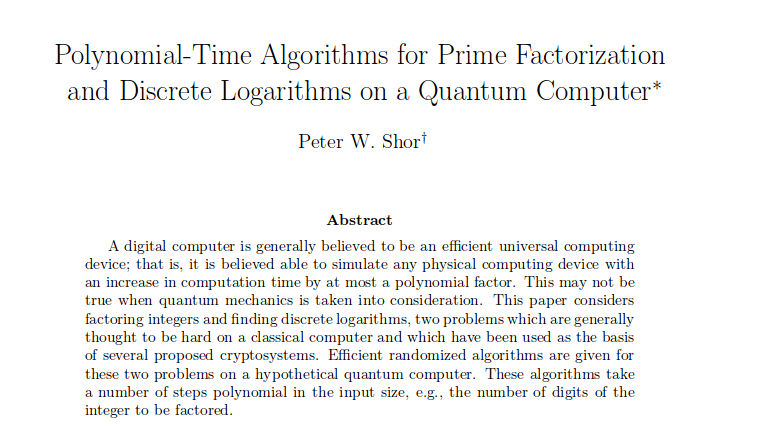
\includegraphics[width=.9\linewidth]{./shor.png}
\end{center}
\end{column}
\end{columns}
\end{frame}

\section{Post-Quantum Cryptography}
\label{sec:org1323478}
\begin{frame}[label={sec:org6599287}]{Post-Quantum Cryptography}
\begin{definition}
Asymmetric cryptographic algorithms run on classical computers that resist attacks using classical and quantum computers.
\end{definition}

\pause

\begin{alertblock}{Note}
Post-quantum cryptography is entirely distinct from quantum cryptography such as a quantum key exchange (QKD). The latter uses quantum effects to achieve security.
\end{alertblock}
\end{frame}

\begin{frame}[label={sec:orga7fa418}]{Post-Quantum Standardisation}
\begin{description}
\item[{NIST}] \textbf{Post Quantum {\color{lightgray}{Competition} }Process}\footnote{“NIST anticipates that the evaluation process for these post-quantum cryptosystems may be significantly more complex than the evaluation of the SHA-3 and AES candidates. … NIST believes that its post-quantum standards development process should not be treated as a competition; in some cases, it may not be possible to make a well-supported judgment that one candidate is ‘better’ than another.“}
\item[{ETSI}] Cyber Working Group for Quantum Safe Cryptography
\item[{ISO}] WG2 Standing Document 8 (SD8): Survey
\item[{IETF}] Standardisation of \textbf{stateful} hash-based signatures, nothing further
\item[{CSA}] Quantum-safe Security Working Group: position papers
\end{description}

\pause

\begin{alertblock}{Status}
Essentially, everyone is waiting for NIST.
\end{alertblock}
\end{frame}

\begin{frame}[label={sec:org9515a65},fragile]{NIST PQC {\color{lightgray}{Competition} }Process}
 \textbf{Timeline}

\begin{itemize}
\item Submission deadline was November 2017.
\item Round 2 selection announced January 2019.
\item Final standard expected 2022-2024.
\end{itemize}

\vspace{1em}

\begin{columns}[t]
\begin{column}{0.5\columnwidth}
\textbf{“Key Exchange”/Key Encapsulation}

\begin{itemize}
\item \texttt{(pk,sk) ← KeyGen()}
\item \texttt{(c,k) ← Encaps(pk)}
\item \texttt{k ← Decaps(c,sk)}
\end{itemize}
\end{column}

\begin{column}{0.5\columnwidth}
\textbf{Digital Signature}

\begin{itemize}
\item \texttt{(vk,sk)  ← KeyGen()}
\item \texttt{s  ← Sig(m, sk)}
\item \texttt{\{0,1\}  ← Verify(s,m,vk)}
\end{itemize}
\end{column}
\end{columns}

\vspace{1em}
\pause

NIST also asked for public-key encryption but this is less important as it can be built generically from a KEM and a block cipher.
\end{frame}

\begin{frame}[label={sec:org0fd3237}]{Security Notions}
\begin{description}
\item[{KEM}] \textbf{IND-CCA}: Given some challenge ciphertext \(c\) and some key \(k\), the adversary gets an oracle to decapsulate (“decrypt”) any other ciphertext but still cannot decide if \(c\) encapsulates (“encrypts”) the key \(k\).

\item[{SIG}] \textbf{EUF-CMA}: Given access to some oracle that signs arbitrary messages, the adversary still cannot produce a valid signature not previously submitted to the signing oracle.
\end{description}

\pause

\begin{block}{Computational Security}
“cannot“ \(\rightarrow\) “computationally infeasible even given access to a quantum computer.”


\pause
\end{block}

\begin{block}{Conditional Security}
“cannot” \(\rightarrow\) “\ldots assuming some mathematical problem is hard on a quantum computer”
\end{block}
\end{frame}

\begin{frame}[label={sec:orgb8f28ef}]{Post-Quantum Candidate Families}
\begin{columns}[t]
\begin{column}{0.4\columnwidth}
\begin{itemize}
\item \alert<1>{Code-based (key encapsulation)}
\item \alert<2>{Multivariate-based (signatures)}
\item \alert<3>{OWF-based (signatures)}
\item \alert<4>{Isogeny-based (key encapsulation)}
\item \alert<5-7>{Lattice-based} (\alert<5,7>{key encapsulation}, \alert<6,7>{signatures})
\end{itemize}
\end{column}

\begin{column}{0.6\columnwidth}
\textbf{NIST PQC 2nd Round}

\begin{description}
\item[{17 KEMs}] \alert<1>{BIKE}, \alert<1>{Classic McEliece}, \alert<5,7>{CRYSTALS-KYBER}, \alert<5,7>{FrodoKEM}, \alert<1>{HQC}, \alert<5,7>{LAC}, \alert<1>{LEDAcrypt}, \alert<5,7>{NewHope}, \alert<5,7>{NTRU}, \alert<5,7>{NTRU Prime}, \alert<1>{NTS-KEM}, \alert<1>{ROLLO}, \alert<5,7>{Round5}, \alert<1>{RQC}, \alert<5,7>{SABER}, \alert<4>{SIKE}, \alert<5,7>{Three Bears}.

\item[{9 SIGs}] \alert<6,7>{CRYSTALS-DILITHIUM}, \alert<6,7>{FALCON}, \alert<2>{GeMSS}, \alert<2>{LUOV}, \alert<2>{MQDSS}, \alert<3>{Picnic}, \alert<6,7>{qTESLA}, \alert<2>{Rainbow}, \alert<3>{SPHINCS+}.
\end{description}
\end{column}
\end{columns}
\end{frame}

\begin{frame}[label={sec:org97a81f6}]{KEM: Code-based}
\textbf{Idea}: Take error-correcting code for up to \(t\) errors. Keep decoding algorithm secret, hide structure of the code.

\begin{columns}[t]
\begin{column}{0.5\columnwidth}
\begin{itemize}
\item Encapsulated key: error vector with \(t\) error indices
\item Most prominent example: McEliece (1978), uses binary Goppa codes
\item Alternatives: QCMDPC codes (e.g. BIKE)
\begin{itemize}
\item Less studied, less conservative, problems with CCA security
\end{itemize}
\end{itemize}
\end{column}

\begin{column}{0.5\columnwidth}
NTS-KEM(13, 136) NIST submission:

\begin{center}
\begin{tabular}{lr}
Key generation & \(\approx\) 240,000,000 cycles\\
Encapsulation & \(\approx\) 280,000 cycles\\
Decapsulation & \(\approx\) 2,000,000 cycles\\
Ciphertext & 253 bytes\\
Public key & 1,419,704 bytes\\
\end{tabular}

\end{center}

\small \url{https://bench.cr.yp.to/results-kem.html}
\end{column}
\end{columns}
\end{frame}

\begin{frame}[label={sec:org4935ac3}]{KEM: Lattice-based}
\textbf{Idea}: Noisy linear algebra mod \(q\) is hard and equivalent to finding short vectors in lattices. Encrypt as solution to noisy linear equations.

\begin{columns}[t]
\begin{column}{0.5\columnwidth}
\begin{itemize}
\item Learning with Errors: given \(\mathbf{A}, \mathbf{b} \equiv \mathbf{A} \cdot \mathbf{s} + \mathbf{e} \bmod q\) where \(\mathbf{e}\) is a vector with small entries, find \(\mathbf{s}\)
\item Most submissions use structured \(\mathbf{A}\)
\begin{itemize}
\item Faster but less conservative
\end{itemize}
\item Frodo uses plain, unstructured LWE
\end{itemize}
\end{column}

\begin{column}{0.5\columnwidth}
Kyber-768 NIST submission:

\begin{center}
\begin{tabular}{lr}
Key generation & \(\approx\)  80,000 cycles\\
Encapsulation & \(\approx\) 100,000 cycles\\
Decapsulation & \(\approx\) 100,000 cycles\\
Ciphertext & 1,152 bytes\\
Public key & 1,088 bytes\\
\end{tabular}

\end{center}

\small \url{https://bench.cr.yp.to/results-kem.html}
\end{column}
\end{columns}
\end{frame}

\begin{frame}[label={sec:org8b10051}]{KEM: SIKE}
\textbf{Idea}: Hard problem is finding a rational map that preserves structure \textbf{between} elliptic curves.

\begin{columns}[t]
\begin{column}{0.5\columnwidth}
\begin{itemize}
\item “Supersingular-Isogeny Diffie-Hellman” (SIDH) proposed in 2011
\item Security related to claw/collision finding, but no reduction from it
\item Rather young construction, more study needed
\end{itemize}
\end{column}

\begin{column}{0.5\columnwidth}
SIKE NIST submission:

\begin{center}
\begin{tabular}{lr}
Key generation & \(\approx\) 13,000,000 cycles\\
Encapsulation & \(\approx\) 20,000,000 cycles\\
Decapsulation & \(\approx\) 20,000,000 cycles\\
Ciphertext & 402 bytes\\
Public key & 378 bytes\\
\end{tabular}

\end{center}

\small \url{https://bench.cr.yp.to/results-kem.html}
\end{column}
\end{columns}
\end{frame}

\begin{frame}[label={sec:org56064d6}]{SIG: OWF-based}
\textbf{Idea}: Start from one-time digital signature based on hash functions. Build Merkle trees on top to produce many-time signature schemes.

\begin{columns}[t]
\begin{column}{0.5\columnwidth}
\begin{itemize}
\item Many tradeoffs possible
\item Secure if there exist collision/pre-image resistant hash functions
\end{itemize}
\end{column}

\begin{column}{0.5\columnwidth}
SPHINCS256 NIST submission:

\begin{center}
\begin{tabular}{lr}
Key generation & \(\approx\)  3,500,000 cycles\\
Signing & \(\approx\) 65,000,000 cycles\\
Verifying & \(\approx\)  1,600,050 cycles\\
Signature & 41,000 bytes\\
Verification key & 1,056 bytes\\
\end{tabular}

\end{center}

\small \url{https://bench.cr.yp.to/results-sign.html}
\end{column}
\end{columns}
\end{frame}

\begin{frame}[label={sec:org8dddfb2}]{SIG: Lattice-based (Hash-and-Sign)}
\textbf{Idea:} Verification key is matrix \(\mathbf{A}\). Hash message \(m\) to vector \(H(m)\). Signature is a \textbf{short} vector \(\vec{s}\) such that \(H(m) = \mathbf{A}\cdot \vec{s}\).

\begin{columns}[t]
\begin{column}{0.5\columnwidth}
\begin{itemize}
\item Can be instantiated from structured and unstructured \(\mathbf{A}\)
\item Typically uses structured lattices
\item Falcon uses NTRU problem: Given \(\mathbf{A} = f/g\) where both \(f,g\) are small. Find \(f\)
\end{itemize}
\end{column}

\begin{column}{0.5\columnwidth}
Falcon-768 NIST submission

\begin{center}
\begin{tabular}{lr}
Key generation & \(\approx\) 43,000,000 cycles\\
Signing & \(\approx\)    930,000 cycles\\
Verifying & \(\approx\)    160,000 cycles\\
Signature & 994 bytes\\
Verification key & 1441 bytes\\
\end{tabular}

\end{center}


\small Falcon submission document
\end{column}
\end{columns}
\end{frame}

\begin{frame}[label={sec:orgb994b4b}]{SIG: MQ-based}
\textbf{Idea:} Hard problem is to find solution to system of \textbf{quadratic} equations in many variables over a finite field.

\begin{columns}[t]
\begin{column}{0.5\columnwidth}
\begin{itemize}
\item All but one submissions use structured systems and assume attacker cannot exploit structure
\item No reduction from standard MQ problem
\item MQDSS reduces to unstructured MQ
\end{itemize}
\end{column}

\begin{column}{0.5\columnwidth}
Rainbow NIST submission

\begin{center}
\begin{tabular}{lr}
Key generation & \(\approx\) 7,000,000 cycles\\
Signing & \(\approx\)    10,000 cycles\\
Verifying & \(\approx\)     6,000 cycles\\
Signature & 42 bytes\\
Verification key & 30,240 bytes\\
\end{tabular}

\end{center}

\small \url{https://bench.cr.yp.to/results-sign.html}
\end{column}
\end{columns}
\end{frame}

\section{The Road Ahead}
\label{sec:orga1d812c}
\begin{frame}[label={sec:orge768bab}]{Parameters Matter}
\begin{quote}
One cannot hope to simply “plug in” a key of 10\textsuperscript{6} or 10\textsuperscript{9} bits into a protocol designed to work for keys of 10\textsuperscript{3} bits and expect it to work as is, and so such results could bring about significant changes to the way we do security over the Internet.  For example, it could lead to a centralization of power, where key exchange will be so expensive that users would share public-keys with only a few large corporations and governments, and smaller companies would have to route their communication through these larger corporations. \footfullcite{EPRINT:Barak17}
\end{quote}
\end{frame}

\begin{frame}[label={sec:orgffa3968}]{PQ Candidates are not DH}
\begin{columns}[t]
\begin{column}{0.5\columnwidth}
Diffie-Hellman is extremely versatile:

\begin{itemize}
\item \alert{Non-Interactive} Key Exchange (NIKE)
\begin{itemize}
\item Bob knows Alice’s long-term pk \(g^a\)
\item Alice knows Bob’s long-term pk \(g^b\)
\item Agree on a shared key before exchanging any messages
\item Expensive to instantiate post-quantum (SIDH-based)
\end{itemize}
\item Oblivious PRF:
\begin{itemize}
\item Alice sends \(h^{r}\) to Bob
\item Bob computes \((h^{r})^b\)
\item Alice computes \((h^{r \cdot b})^{(1/r)}\)
\item Not clear how to instantiate post-quantum
\end{itemize}
\end{itemize}
\end{column}

\begin{column}{0.5\columnwidth}
Lattices are extremely versatile:

\begin{itemize}
\item Fully-Homomorphic Encryption (FHE)
\begin{itemize}
\item Computing on encrypted data
\item Only from lattices
\end{itemize}
\item Identity-Based Encryption (IBE)
\begin{itemize}
\item Names \alert{are} the public keys
\end{itemize}
\item Attribute-Based Encryption (ABE)
\begin{itemize}
\item Encrypt to all doctors in an organisation etc.
\end{itemize}
\item \ldots
\end{itemize}
\end{column}
\end{columns}
\end{frame}

\begin{frame}[label={sec:org49baec5}]{Alternatives: QKD?}
\begin{quote}
QKD: has fundamental practical limitations; does not address large parts of the security problem; is poorly understood in terms of potential attacks.

By contrast, post-quantum public key cryptography appears to offer much more effective mitigations for real-world communications systems from the threat of future quantum computers.\footfullcite{NCSC:QKD16}
\end{quote}

\begin{itemize}
\item attacks on implementations/instantiations
\item limited range, dedicated hardware
\item limited speed \(\rightarrow\) keys then used in AES
\item authentication required: MAC or digital signature
\end{itemize}
\end{frame}

\begin{frame}[label={sec:org6f41df4}]{The Road Ahead}
\begin{itemize}
\item We need to understand the underlying hard problems better
\item Resistance to side-channel attacks
\item Efficient, safe implementations
\item How fast is fast enough? How small is small enough?
\item How do existing protocols interact with post-quantum primitives? Should we change protocols?
\end{itemize}
\end{frame}

\begin{frame}[label={sec:orge5669fb}]{Don’t Jump the Gun!}
\begin{itemize}
\item Temptation to pick one of the NIST candidates as drop-in replacement for deployment in existing protocols \alert{now}

\item This is a terrible idea!
\begin{itemize}
\item mediocre performance
\item non-optimal security properties
\end{itemize}

\item Bad cryptography is very hard to get rid of (think MD5)

\item Will also need to think carefully about changes to protocols

\item Let’s get this one right!
\end{itemize}

\pause

\begin{block}{Proof of Concept Code}
\ldots even worse idea: pick \textbf{source code} of one of the NIST candidates to deploy
\end{block}
\end{frame}

\begin{frame}[label={sec:org6ec1bb4},standout]{Fin}
\begin{center}
\Huge \alert{Thank You}
\end{center}
\end{frame}

\begin{frame}[allowframebreaks]{References}
\renewcommand*{\bibfont}{\scriptsize}
\printbibliography[heading=none]
\end{frame}
\end{document}